\documentclass{theme-2614084}
\usepackage{hyperref}
\usepackage{bookmark}
\usepackage{minted}

\usepackage{hyperref}

% =============================================
% Part 0 信息
% =============================================

\mathsetup{
  % 学生姓名
  student-name = {某同学},
  % 学号
  student-id = {2021xxxx},
  % 院系
  department = {电子与信息工程学院},
  % 专业
  experiment = {实验4 CMOS与非门版图设计},
  % 专业年级
  major = {集成电路设计与集成系统},
  % 日期
  % date = {\today},
}

\begin{document}

% =============================================
% Part 1  封面
% =============================================

\makecover

% =============================================
% Part 2 主文档
% =============================================

\section{实验目的}

\begin{enumerate}
  \item 熟悉 virtuoso editing 设计窗口及操作,熟悉 LSW 窗口
  \item 理解设计库、技术库
  \item 了解 SMIC0.18um 工艺规则
  \item 认识 DRC 设计规则检查,排除错误
\end{enumerate}

\section{实验环境}

\begin{enumerate}
  \item 硬件: PC 机、服务器
  \item 环境:Unix 操作系统、Cadence Virtuoso Editing 版图设计软件
\end{enumerate}

\section{实验内容与步骤}

% (注:按照内容,有截图和说明)

\subsection{实验内容}

\begin{enumerate}
  \item 按照设计规则进行CMOS与非门的版图设计。
  \item 进行CMOS与非门的DRC、LVS检查,生成GDS 文件。
\end{enumerate}

\subsection{实验步骤}

\subsubsection{准备工作}

在新的terminal里面,将当前目录调整到:

\begin{minted}[
  frame=lines,
  framesep=2mm,
  baselinestretch=1.2,
  fontsize=\small,
]{bash}
/qixin/public/layout_libs/smic180/pdk/smic18ee_2P5M_20100920
\end{minted}

类似地,输入 

\begin{minted}[
  frame=lines,
  framesep=2mm,
  baselinestretch=1.2,
  fontsize=\small,
]{bash}
cp cds.lib /qixin/home/stu92/2021xxxx
\end{minted}

复制 cds.lib 文件到刚刚建立的 

\begin{minted}[
  frame=lines,
  framesep=2mm,
  baselinestretch=1.2,
  fontsize=\small,
]{bash}
/qixin/home/stu92/2021xxxx
\end{minted}

文件夹当中。

回到第一个terminal窗口中,输入ls,确认cds.lib这两个文件已被复制到 /qixin/home/stu92/2021xxxx 文件夹当中。

输入gvim cds.lib 并如图所示更新cds.lib的文本内容

\begin{minted}[
  frame=lines,
  framesep=2mm,
  baselinestretch=1.2,
  fontsize=\small,
]{bash}
DEFINE smic18ee /qixin/public/layout_libs/smic180/pdk/smic18ee_2P5M_20100920/smic18ee
DEFINE schematic /qixin/public/layout_libs/smic180/schematic
\end{minted}

\begin{figure}[H]
  \centering
  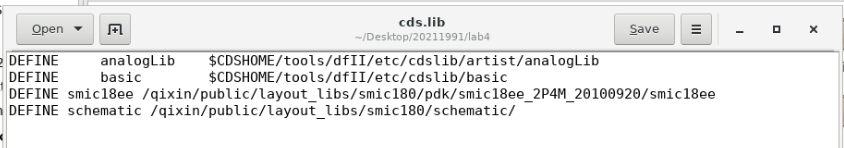
\includegraphics[width=0.6\linewidth]{1-prepare/update-cdslib.png}
  \caption{update cds.lib}
\end{figure}

输入virtuoso\& 并回车,打开virtuoso

新建 Library,并配置 Attach 技术库

\begin{figure}[htbp]
  \centering\begin{minipage}[t]{0.48\textwidth}
      \centering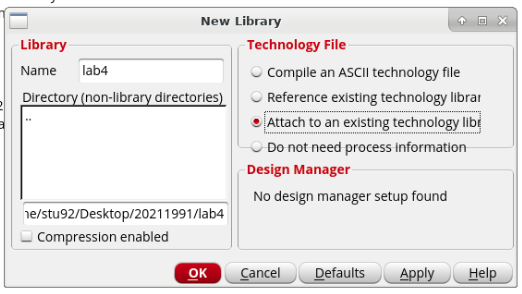
\includegraphics[width=0.9\textwidth]{1-prepare/create-new-library.png}
      \caption{create new library}
  \end{minipage}
  \centering\begin{minipage}[t]{0.48\textwidth}
      \centering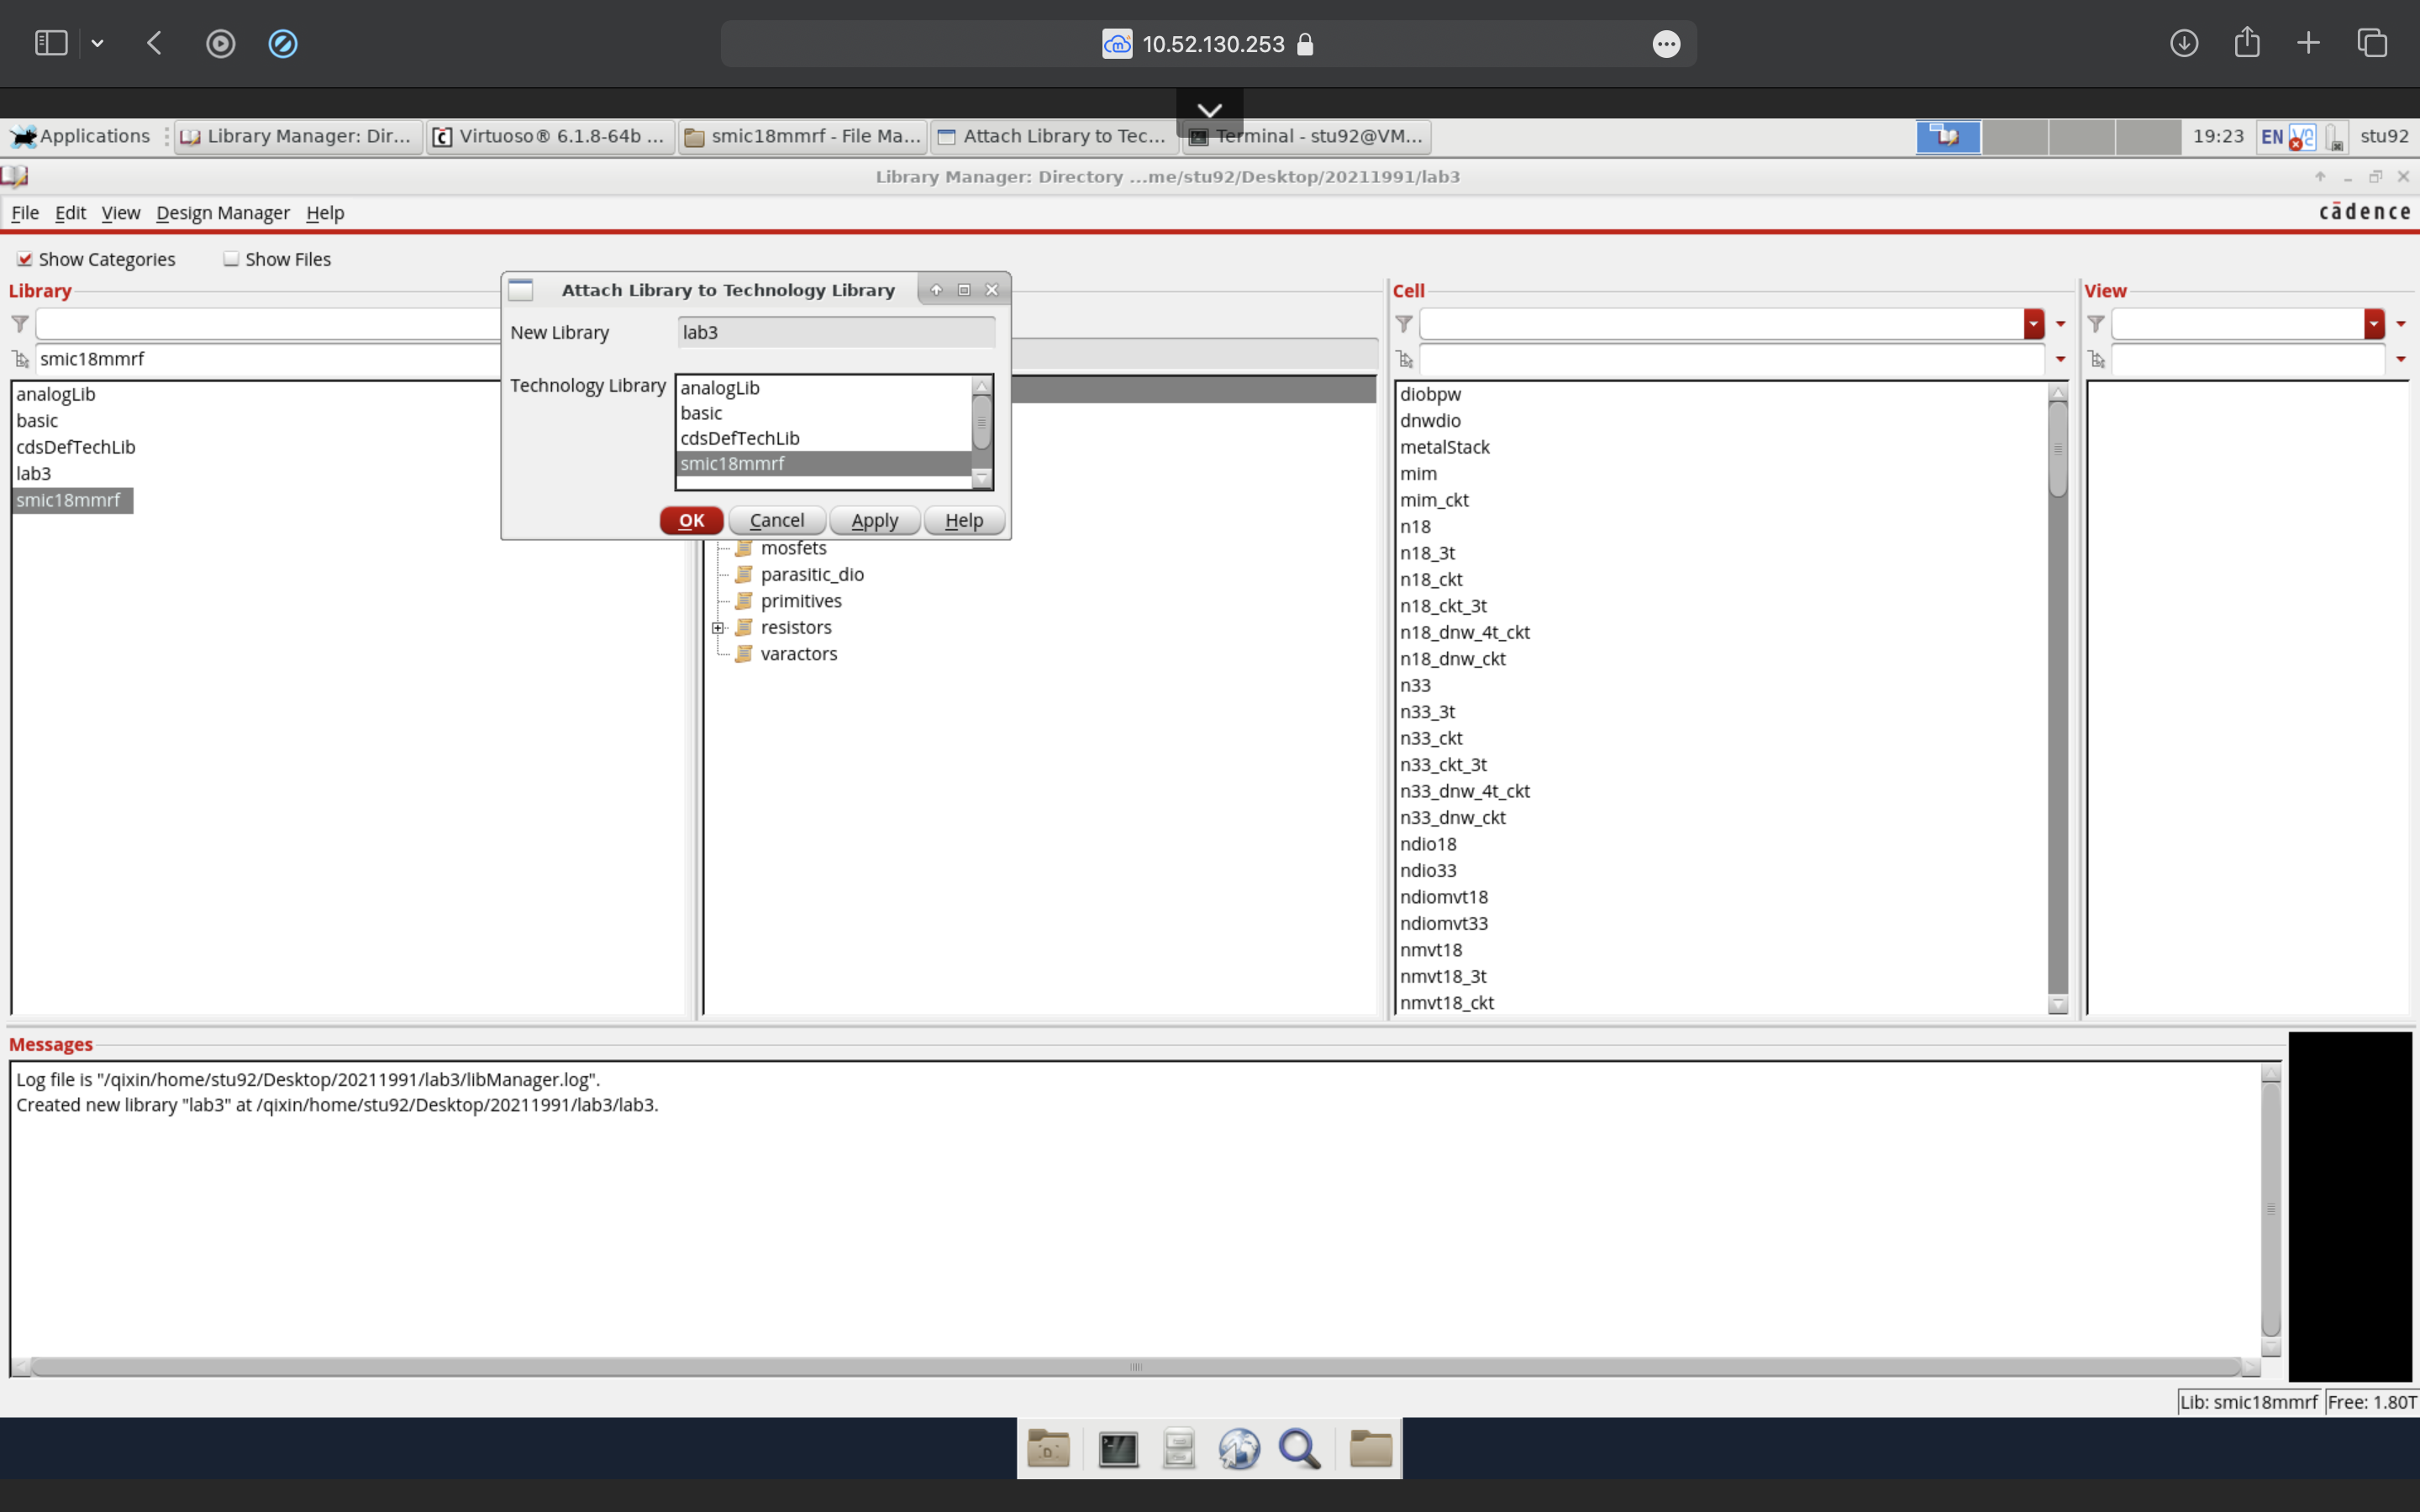
\includegraphics[width=0.9\linewidth]{1-prepare/create-new-library-attach.png}
      \caption{attach technology library}
  \end{minipage}
\end{figure}

\subsubsection{与非门的原理图(schematic)}

可以看到一套现成的与非门的原理图

\begin{figure}[H]
  \centering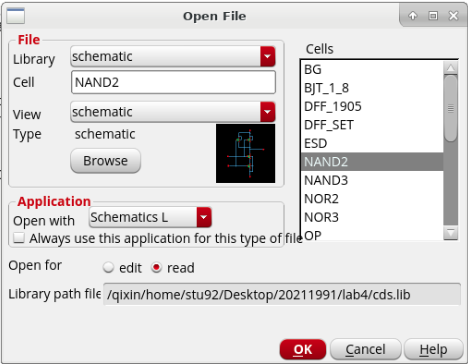
\includegraphics[width=0.6\linewidth]{2-nand2-schematic/open-nand2-in-schematic.png}
  \caption{open nand2 in schematic}
\end{figure}

\subsubsection{与非门的版图(layout)}

Lanuch->layout XL

\begin{figure}[H]
  \centering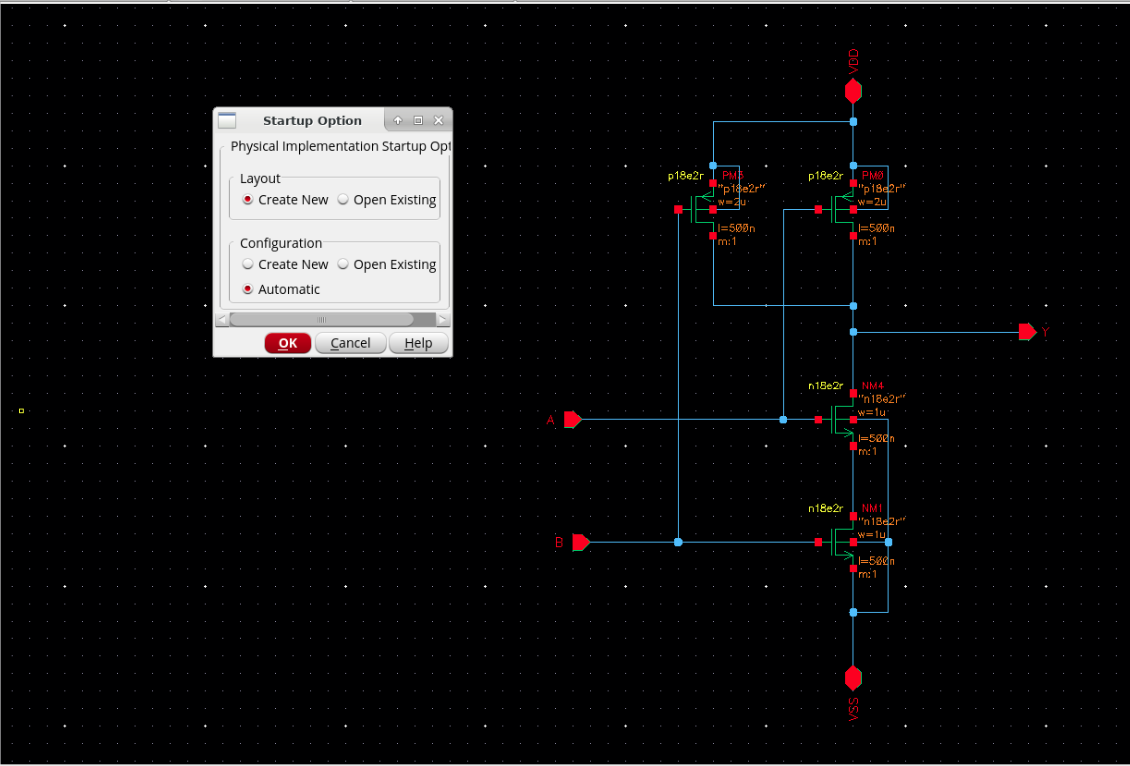
\includegraphics[width=0.6\linewidth]{3-nand2-layout/create-new-layout-1.png}
  \caption{create new layout}
\end{figure}

\begin{figure}[H]
  \centering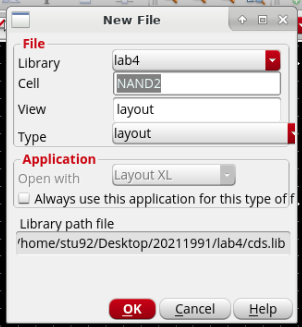
\includegraphics[width=0.6\linewidth]{3-nand2-layout/create-new-layout-2.png}
  \caption{create new layout}
\end{figure}

点击 \texttt{Generate All From Source} 生成版图,此处开自动就行。

\begin{figure}[H]
  \centering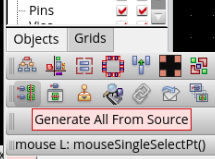
\includegraphics[width=0.6\linewidth]{3-nand2-layout/generate-all-from-source-1.png}
  \caption{click generate all from source}
\end{figure}

取消勾选 \texttt{PR Boundary},点击 \texttt{OK}

\begin{figure}[H]
  \centering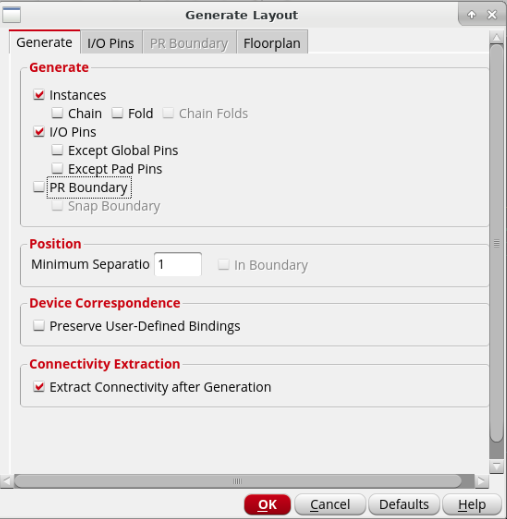
\includegraphics[width=0.6\linewidth]{3-nand2-layout/generate-all-from-source-2.png}
  \caption{settings for generate all from source}
\end{figure}

在 \texttt{I/O Pins} 中,按照下图进行设置,勾选 \texttt{Create Label As} 选项,点击 \texttt{Options} ,按照下图进行设置

\begin{figure}[htbp]
  \centering\begin{minipage}[t]{0.48\textwidth}
      \centering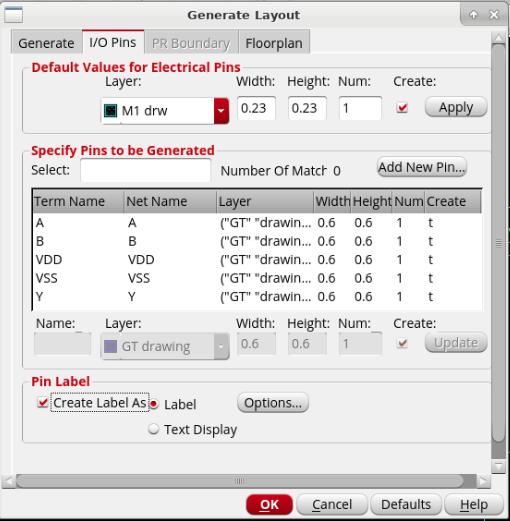
\includegraphics[width=0.9\textwidth]{3-nand2-layout/generate-all-from-source-3.png}
      \caption{settings for generate all from source}
  \end{minipage}
  \centering\begin{minipage}[t]{0.48\textwidth}
      \centering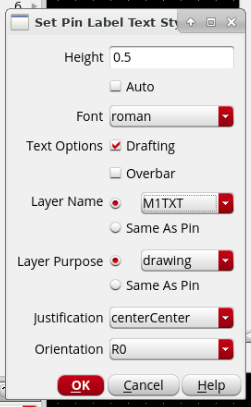
\includegraphics[width=0.9\linewidth]{3-nand2-layout/generate-all-from-source-4.png}
      \caption{settings for generate all from source}
  \end{minipage}
\end{figure}

点击 \texttt{Options -> Display},按照下图进行设置

\begin{figure}[H]
  \centering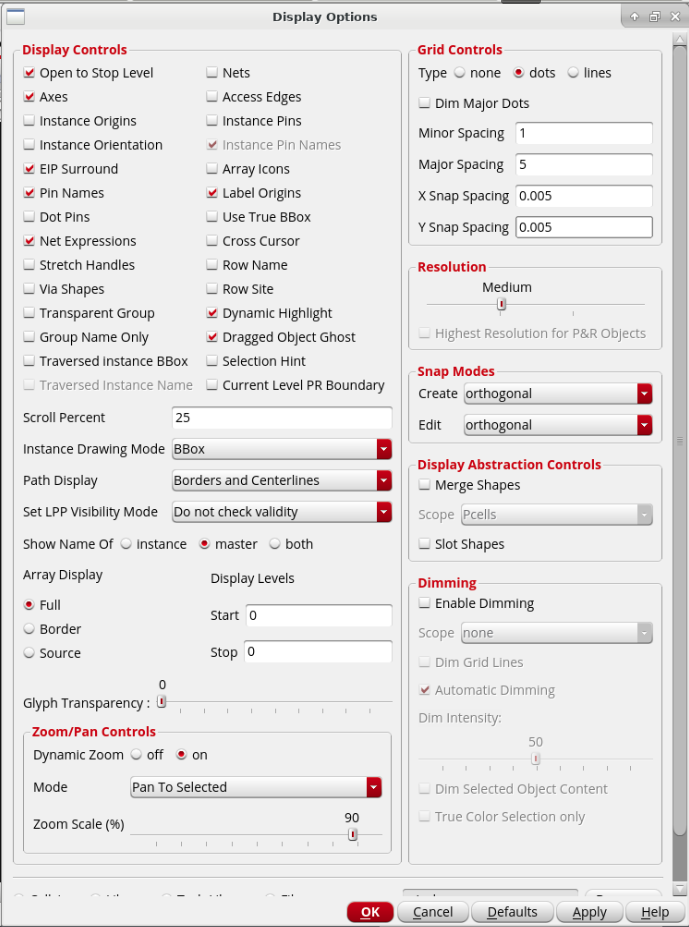
\includegraphics[width=0.6\linewidth]{3-nand2-layout/display-options.png}
  \caption{display options}
\end{figure}

\texttt{Shift+F} 在 Virtuoso Layout 中,按下 Shift + F 键可以将视图展开为实例的子布局,以显示其组成的各个层

删掉红框框出的部分

\begin{figure}[H]
  \centering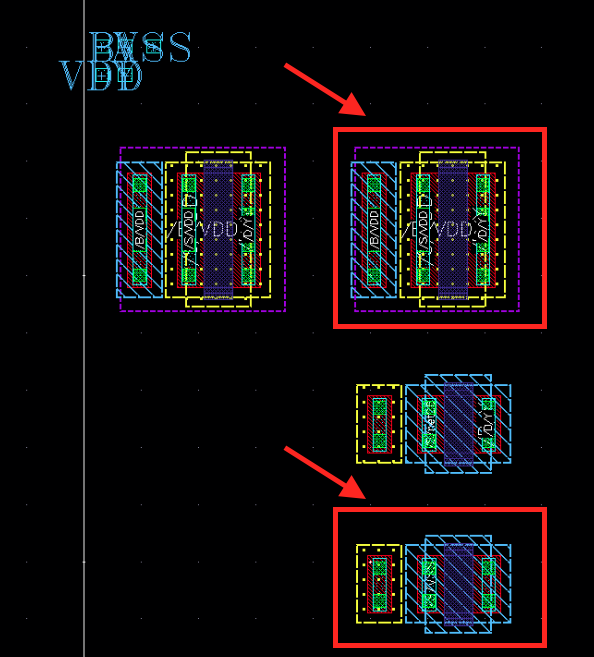
\includegraphics[width=0.6\linewidth]{3-nand2-layout/delete-part.png}
  \caption{delete part}
\end{figure}

选中左上的这个器件,按右键,点properties

将其中 Parameter -> Fingers 的值改为 2,勾选 \texttt{Top Tap} 随后 Apply

\begin{figure}[htbp]
  \centering\begin{minipage}[t]{0.48\textwidth}
      \centering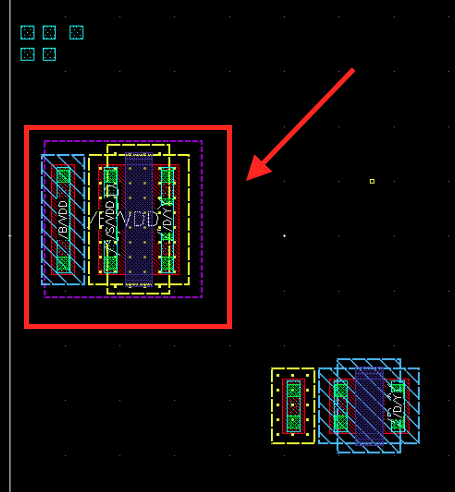
\includegraphics[width=0.9\textwidth]{3-nand2-layout/PM3-p18e2r-properties-1.png}
      \caption{PM3-p18e2r properties}
  \end{minipage}
  \centering\begin{minipage}[t]{0.48\textwidth}
      \centering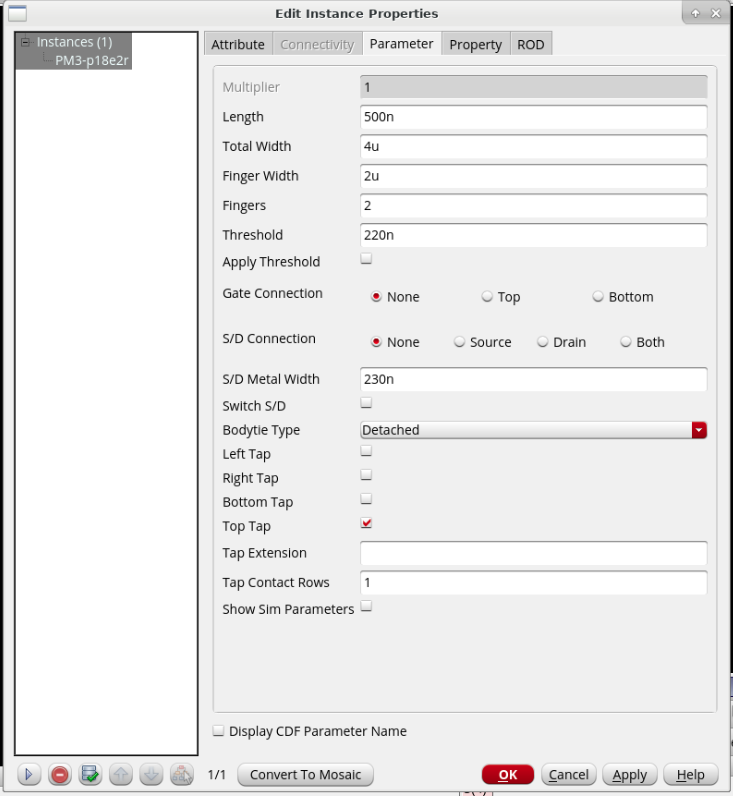
\includegraphics[width=0.9\linewidth]{3-nand2-layout/PM3-p18e2r-properties-2.png}
      \caption{PM3-p18e2r properties}
  \end{minipage}
\end{figure}

选中红框框出的部分,按右键,点properties

将其中 Parameter -> Fingers 的值改为 2,勾选 \texttt{Bottom Tap} 随后 Apply

\begin{figure}[htbp]
  \centering\begin{minipage}[t]{0.48\textwidth}
      \centering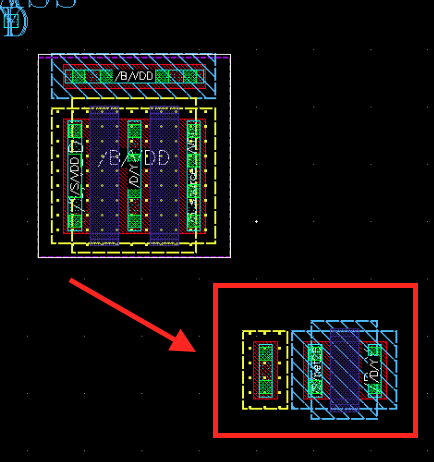
\includegraphics[width=0.9\textwidth]{3-nand2-layout/NM4-n18e2r-properties-1.png}
      \caption{NM4-n18e2r properties}
  \end{minipage}
  \centering\begin{minipage}[t]{0.48\textwidth}
      \centering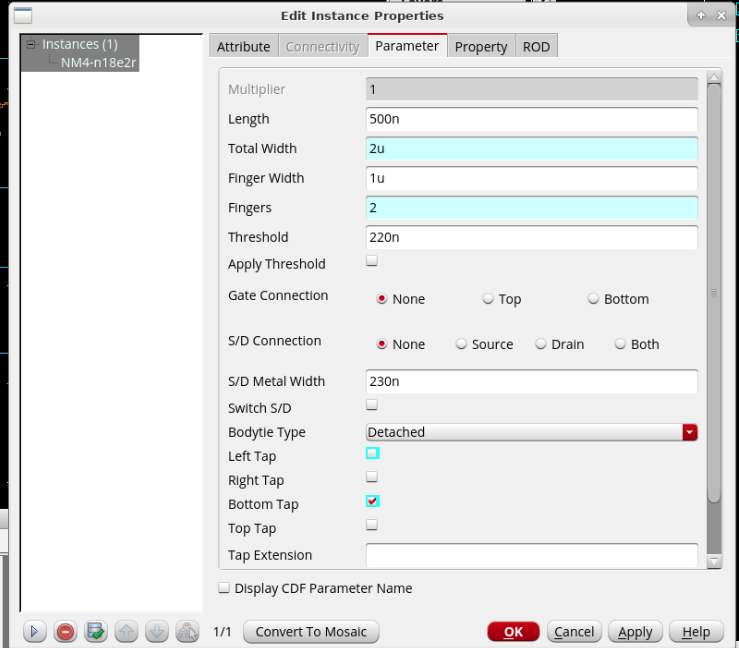
\includegraphics[width=0.9\linewidth]{3-nand2-layout/NM4-n18e2r-properties-2.png}
      \caption{NM4-n18e2r properties}
  \end{minipage}
\end{figure}

按一下k之后,如图所示画出两条标记线

\begin{figure}[H]
  \centering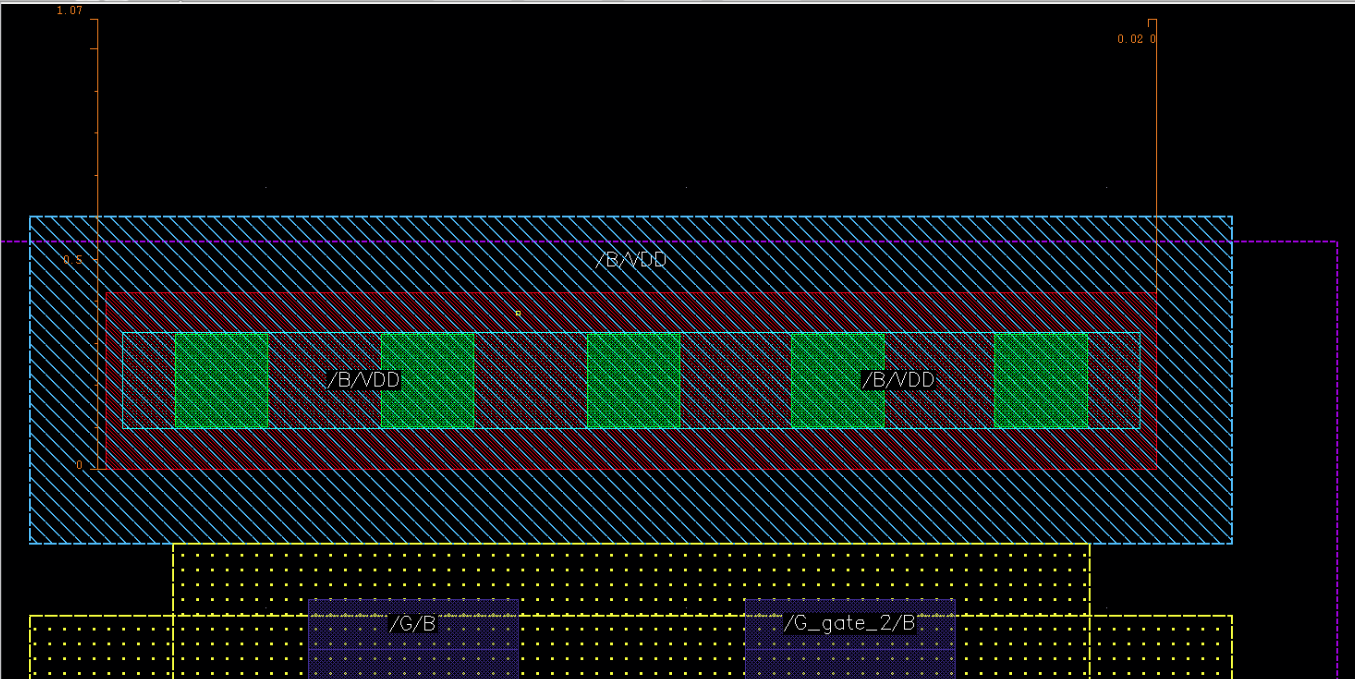
\includegraphics[width=0.6\linewidth]{3-nand2-layout/draw-ruler-1.png}
  \caption{draw ruler}
\end{figure}

\begin{figure}[H]
  \centering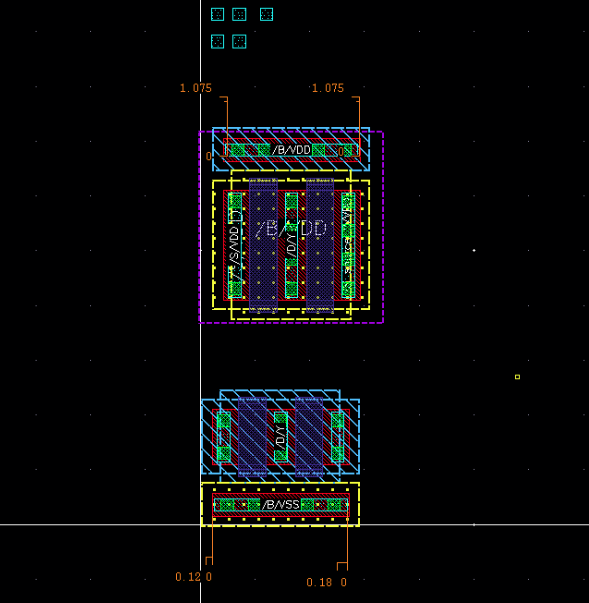
\includegraphics[width=0.6\linewidth]{3-nand2-layout/draw-ruler-2.png}
  \caption{draw ruler}
\end{figure}

右键点击如图所示空白,在随后出现的菜单中,勾选 Guardring

NOTES: \textbf{此处我的设置界面和Courseware上的不太一样,暂时不清楚有什么影响}

点一下刚画的这个标记线,然后开始画Guardring

画出如下图这样

\begin{figure}[htbp]
  \centering\begin{minipage}[t]{0.48\textwidth}
      \centering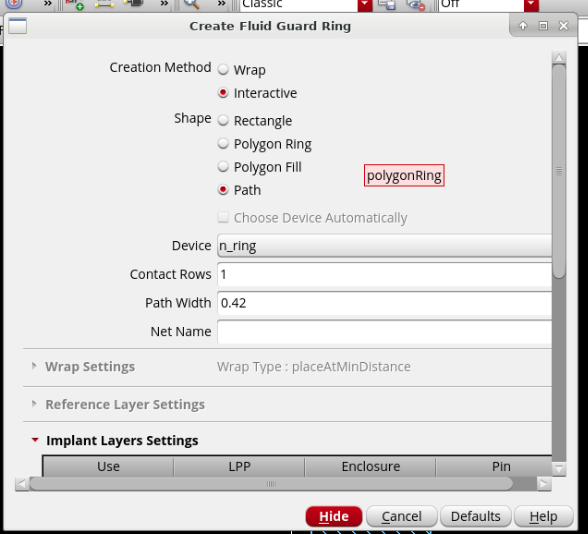
\includegraphics[page=1, width=0.9\textwidth]{3-nand2-layout/create-fluid-guard-ring-1.png}
      \caption{create fluid guardring}
  \end{minipage}
  \centering\begin{minipage}[t]{0.48\textwidth}
      \centering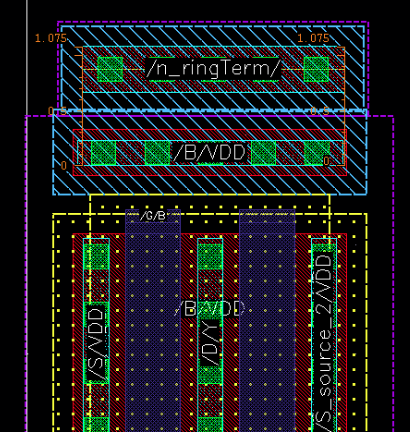
\includegraphics[width=0.9\linewidth]{3-nand2-layout/create-fluid-guard-ring-2.png}
      \caption{create fluid guardring}
  \end{minipage}
\end{figure}

\begin{figure}[htbp]
  \centering\begin{minipage}[t]{0.48\textwidth}
      \centering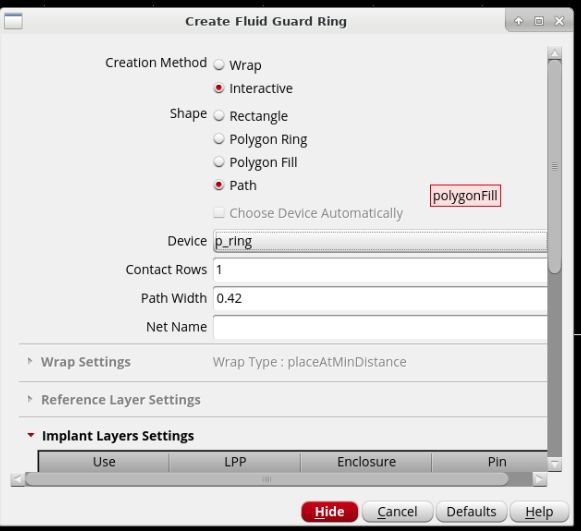
\includegraphics[width=0.9\linewidth]{3-nand2-layout/create-fluid-guard-ring-3.png}
      \caption{create fluid guardring}
  \end{minipage}
  \centering\begin{minipage}[t]{0.48\textwidth}
      \centering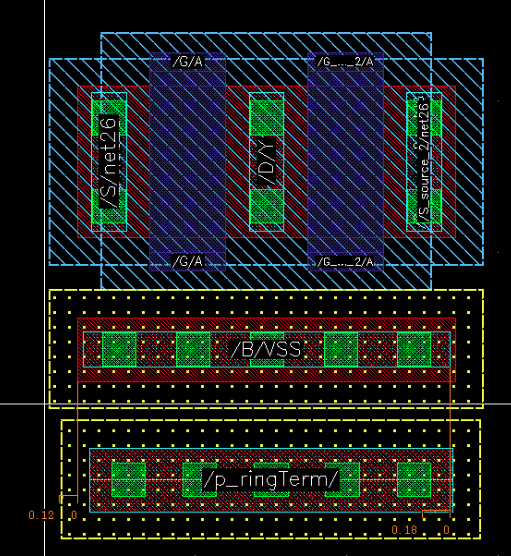
\includegraphics[width=0.9\linewidth]{3-nand2-layout/create-fluid-guard-ring-4.png}
      \caption{create fluid guardring}
  \end{minipage}
\end{figure}

选中 PM3-p18e2r,按右键,点properties,取消勾选 \texttt{Top Tap},Apply

选中 NM4-n18e2r,按右键,点properties,取消勾选 \texttt{Bottom Tap},Apply

保留刚刚自己画的Guardring

如图接线

\begin{figure}[H]
  \centering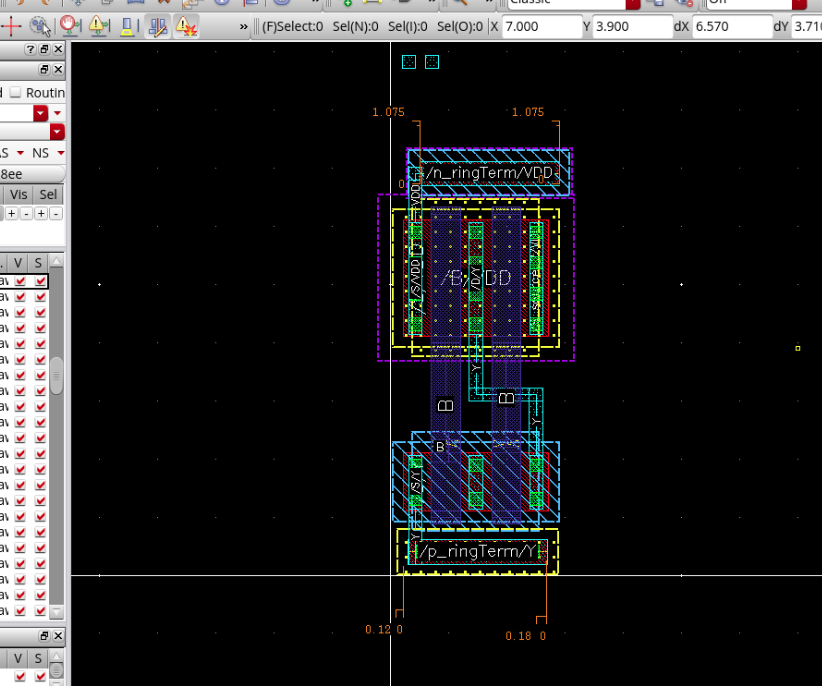
\includegraphics[width=0.6\linewidth]{3-nand2-layout/create-connection-1.png}
  \caption{create connection}
\end{figure}

按一下 \texttt{o} 键 -- 打孔

\begin{figure}[H]
  \centering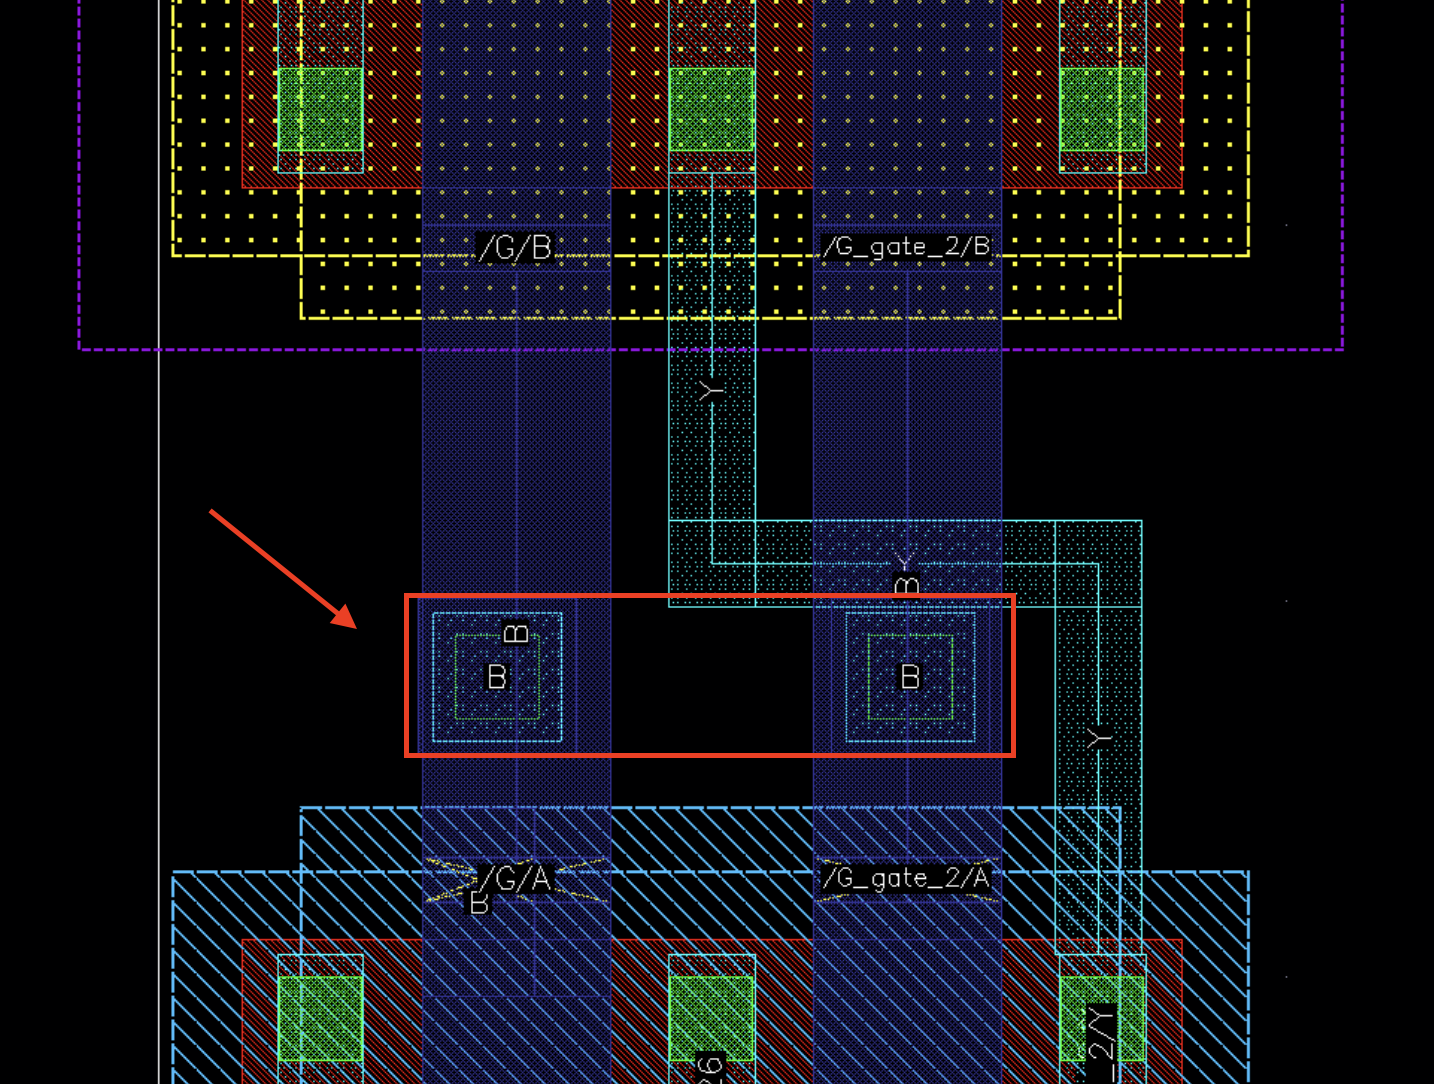
\includegraphics[width=0.6\linewidth]{3-nand2-layout/create-via-1.png}
  \caption{create via}
\end{figure}

放置label

NOTES: \textbf{不知道这个 label 咋放,之后补充}

\subsection{与非门的DRC}

点击 \texttt{Calibre -> Run nmDRC}

点击 \texttt{Rule},\texttt{DRC Rules File},路径选择

\begin{minted}[
  frame=lines,
  framesep=2mm,
  baselinestretch=1.2,
  fontsize=\small,
]{bash}
/qixin/public/layout_libs/smic180/calibre/drc/
\end{minted}

\begin{figure}[htbp]
  \centering\begin{minipage}[t]{0.48\textwidth}
      \centering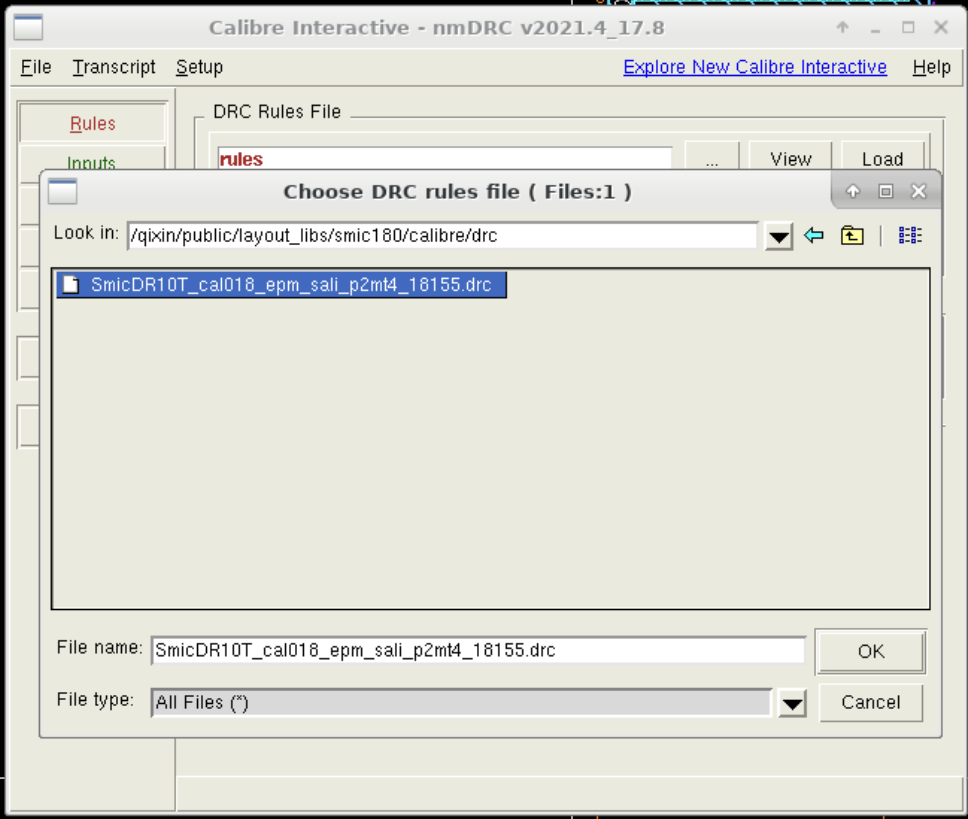
\includegraphics[width=0.9\linewidth]{4-nand2-drc/choose-drc-rules-file.png}
      \caption{choose drc rules file}
  \end{minipage}
  \centering\begin{minipage}[t]{0.48\textwidth}
      \centering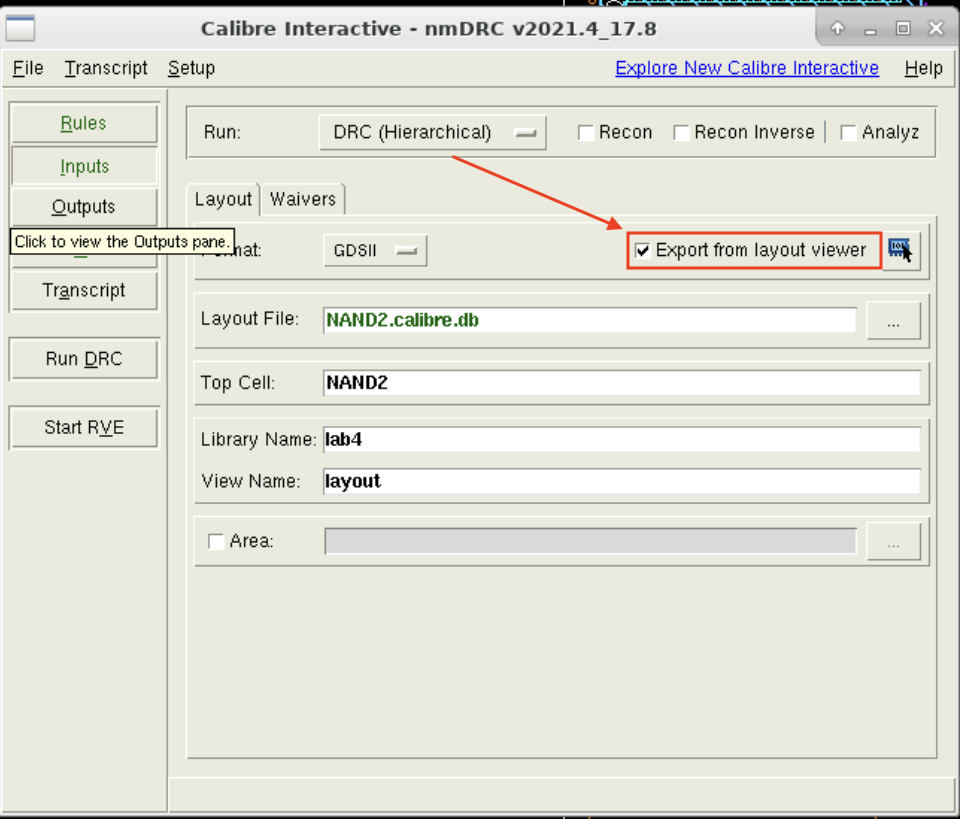
\includegraphics[width=0.9\linewidth]{4-nand2-drc/set-input.png}
      \caption{set input}
  \end{minipage}
\end{figure}

点击 \texttt{Run DRC},得到如下结果

\begin{figure}[H]
  \centering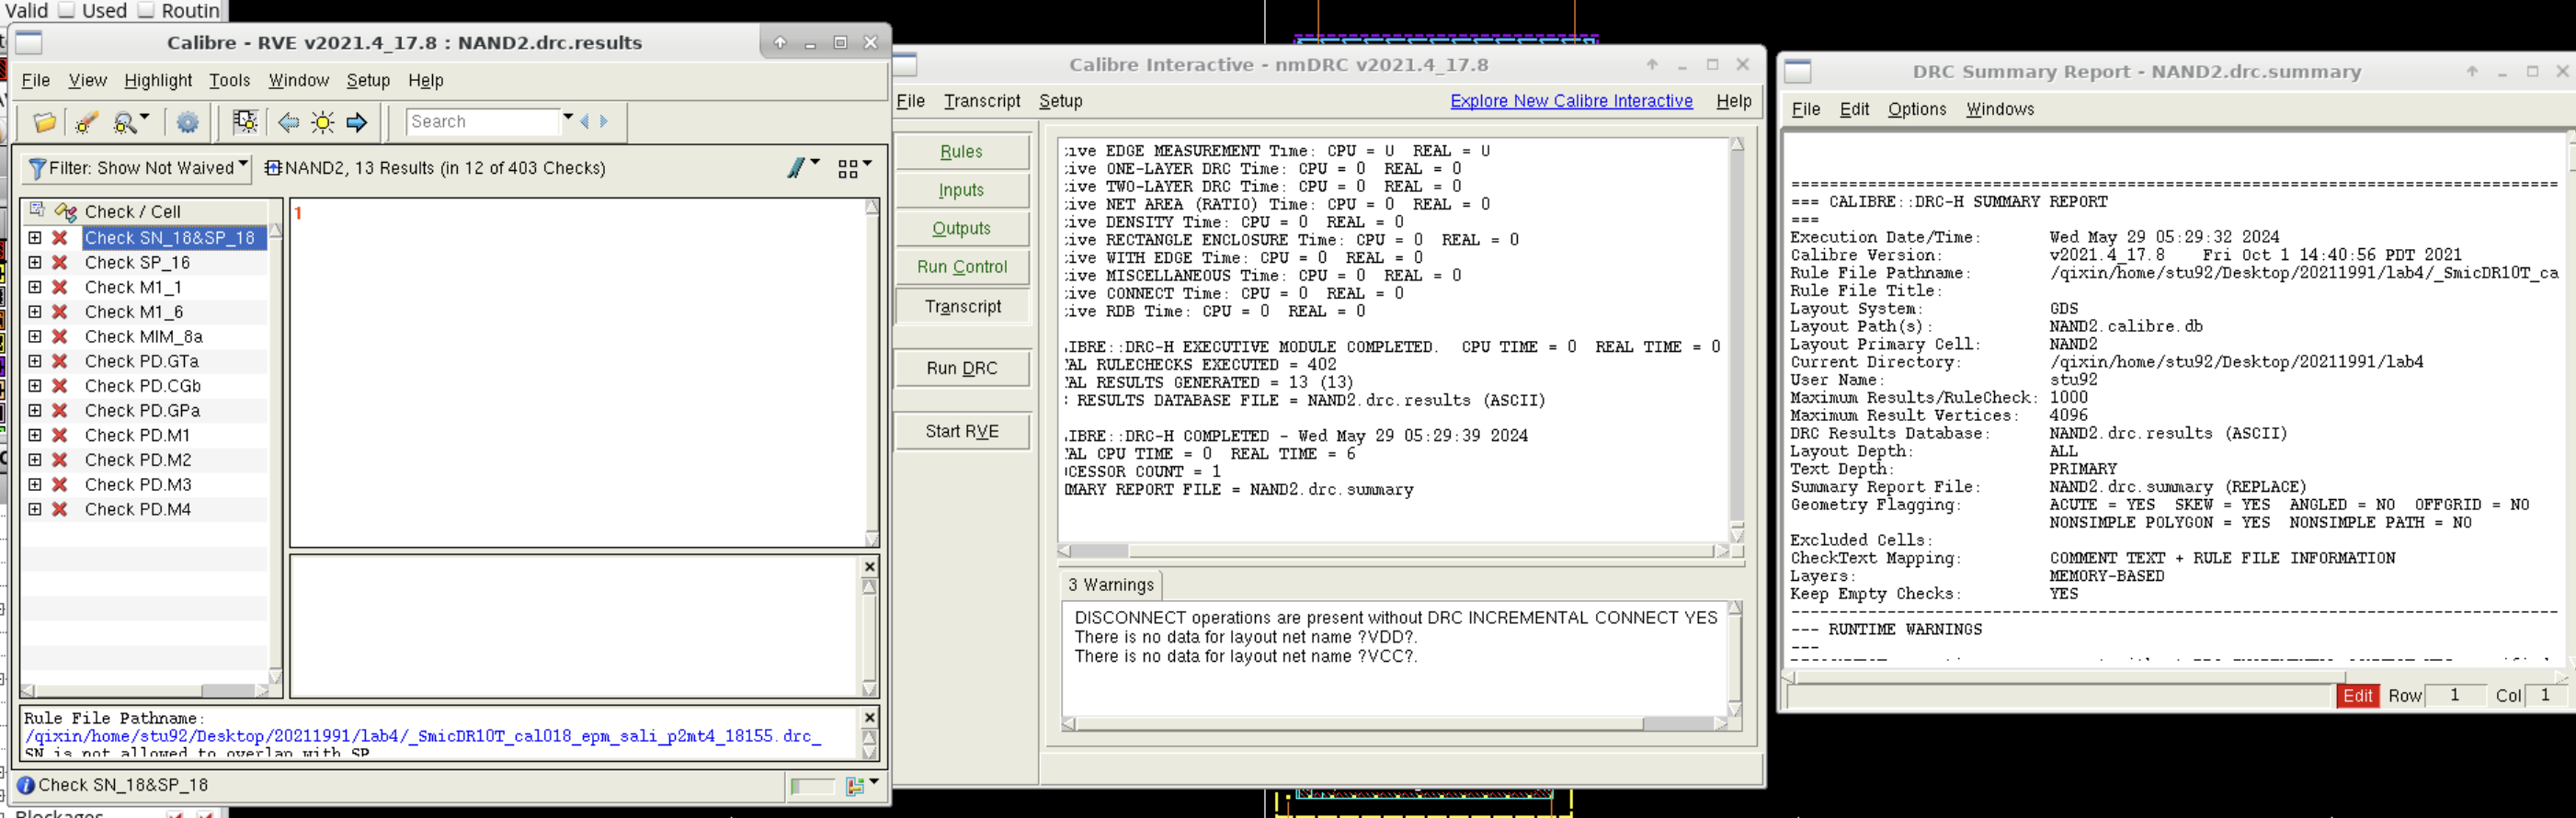
\includegraphics[width=0.6\linewidth]{4-nand2-drc/drc-report-2.png}
  \caption{drc report}
\end{figure}

选择 show not waived
可以看到,有一个 \texttt{Check\_M1\_6} 详情是说:M1区域的最小面积是0.2um,也就是说,我们现在的M1区域的面积还不到0.2um,我们需要像下图那样调整一下。

\begin{figure}[H]
  \centering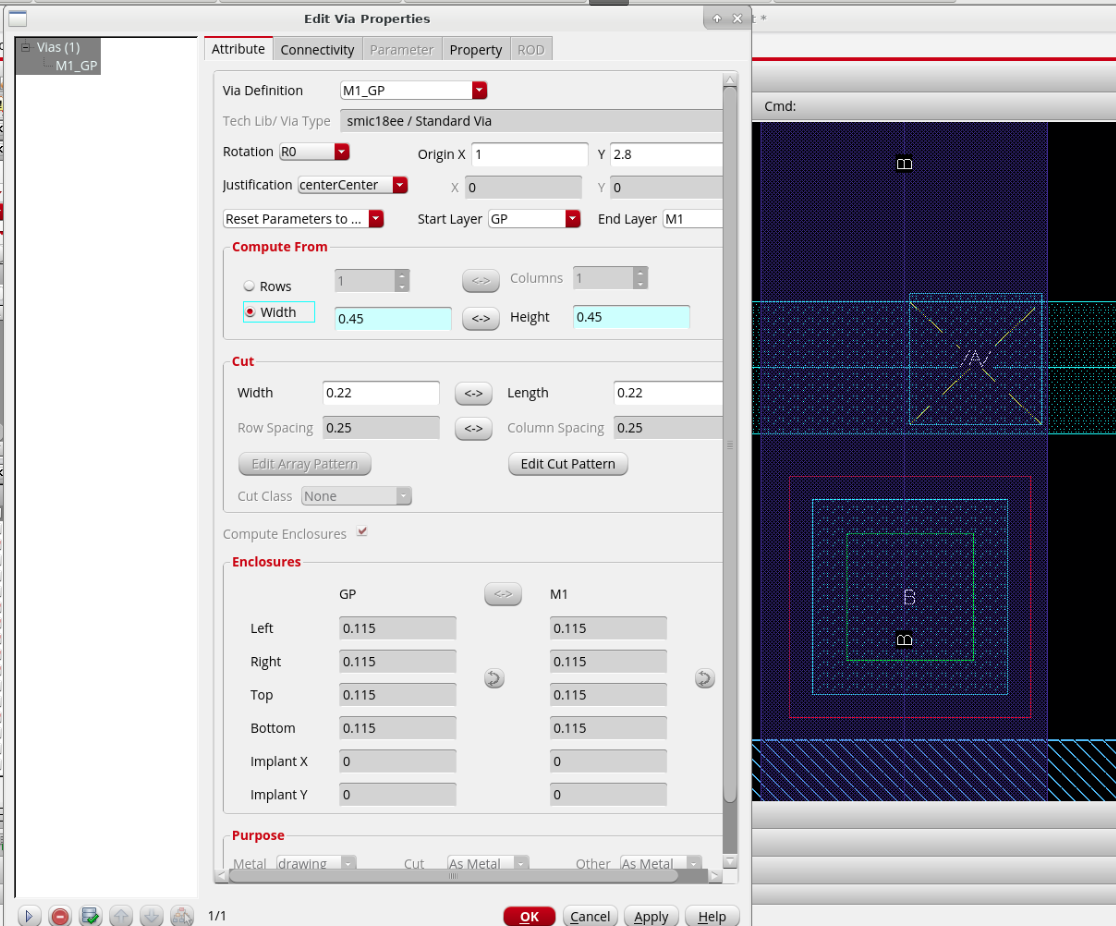
\includegraphics[width=0.6\linewidth]{4-nand2-drc/edit-via-properties.png}
  \caption{edit via properties}
\end{figure}

修改后,再次点击 \texttt{Calibre -> Run nmDRC},选择 show not waived,可以看到,前面那个 \texttt{Check\_M1\_6} ,现在已经没有了,说明我们调整过后,这一项符合要求,不再提示错误。

\begin{figure}[H]
  \centering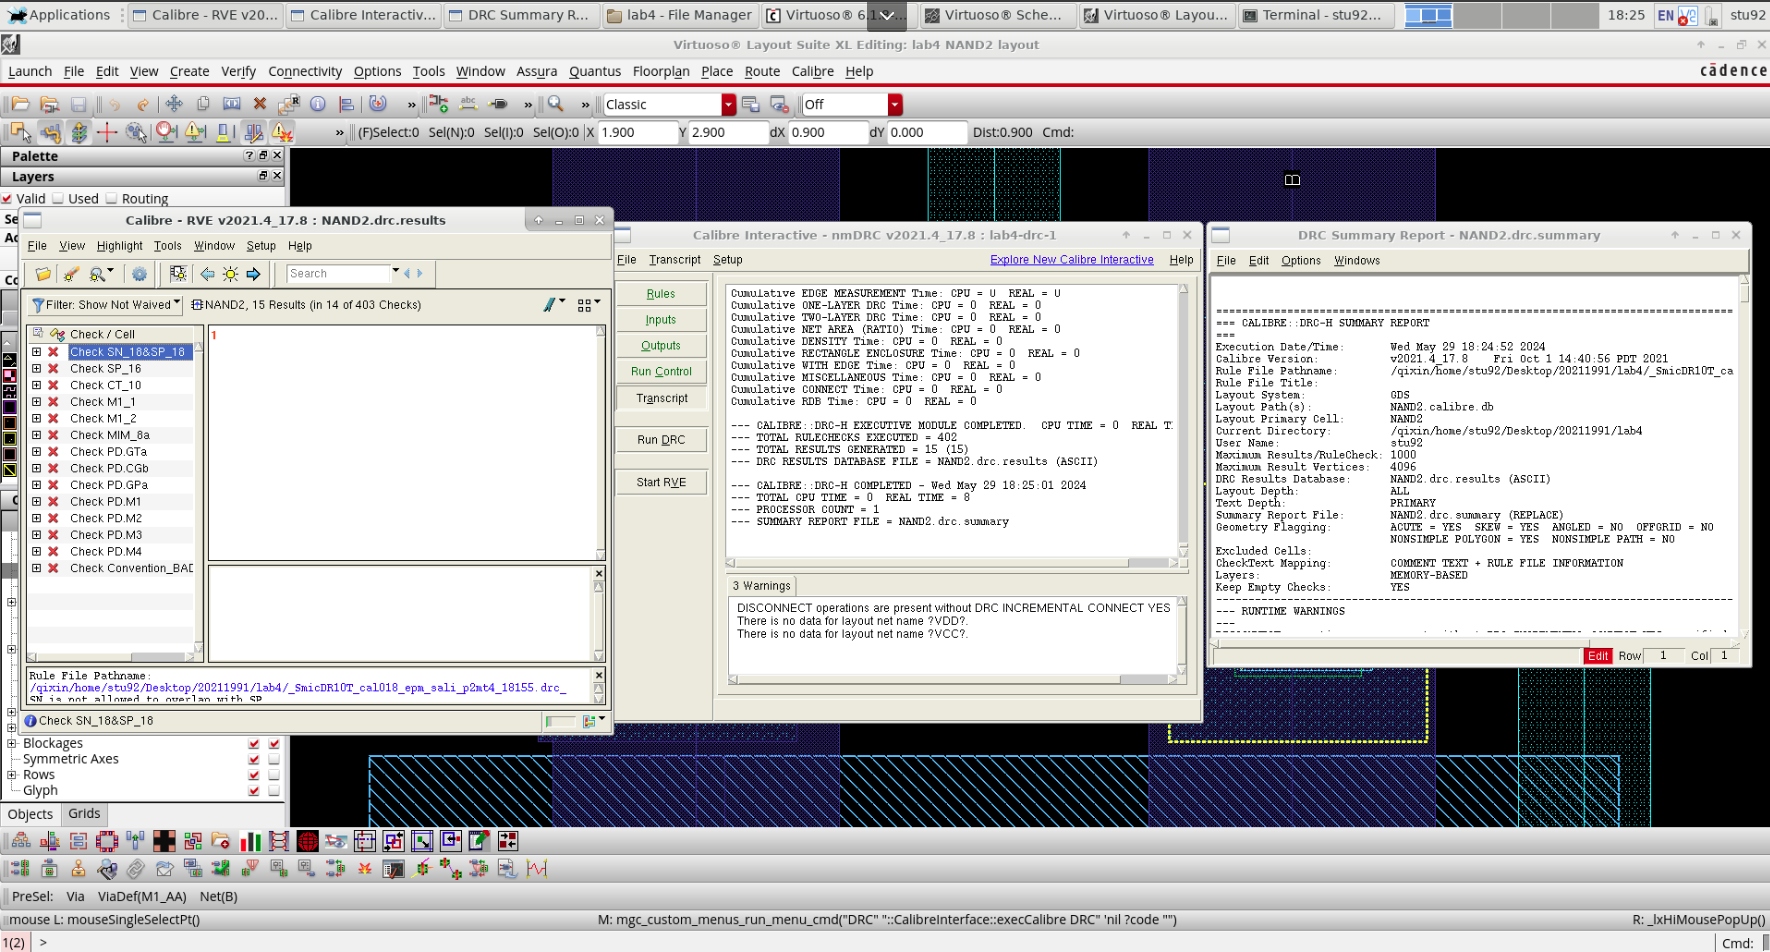
\includegraphics[width=0.6\linewidth]{4-nand2-drc/drc-report-3.png}
  \caption{drc report}
\end{figure}

\subsection{与非门的LVS}

点击 \texttt{Rule},\texttt{DRC Rules File},路径选择

\begin{figure}[H]
  \centering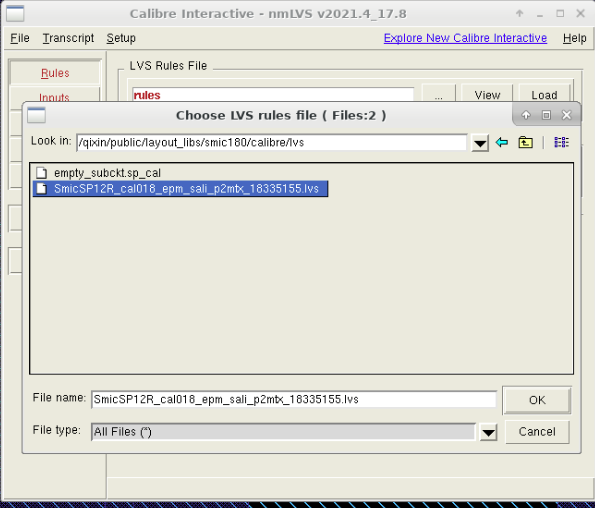
\includegraphics[width=0.6\linewidth]{5-nand2-lvs/choose-lvs-rules-file.png}
  \caption{choose lvs rules file}
\end{figure}

点击 \texttt{Calibre -> Run nmLVS}

如果出现如图所示的X,没看到笑脸,那需要我们看一下错误在哪里。

\begin{figure}[H]
  \centering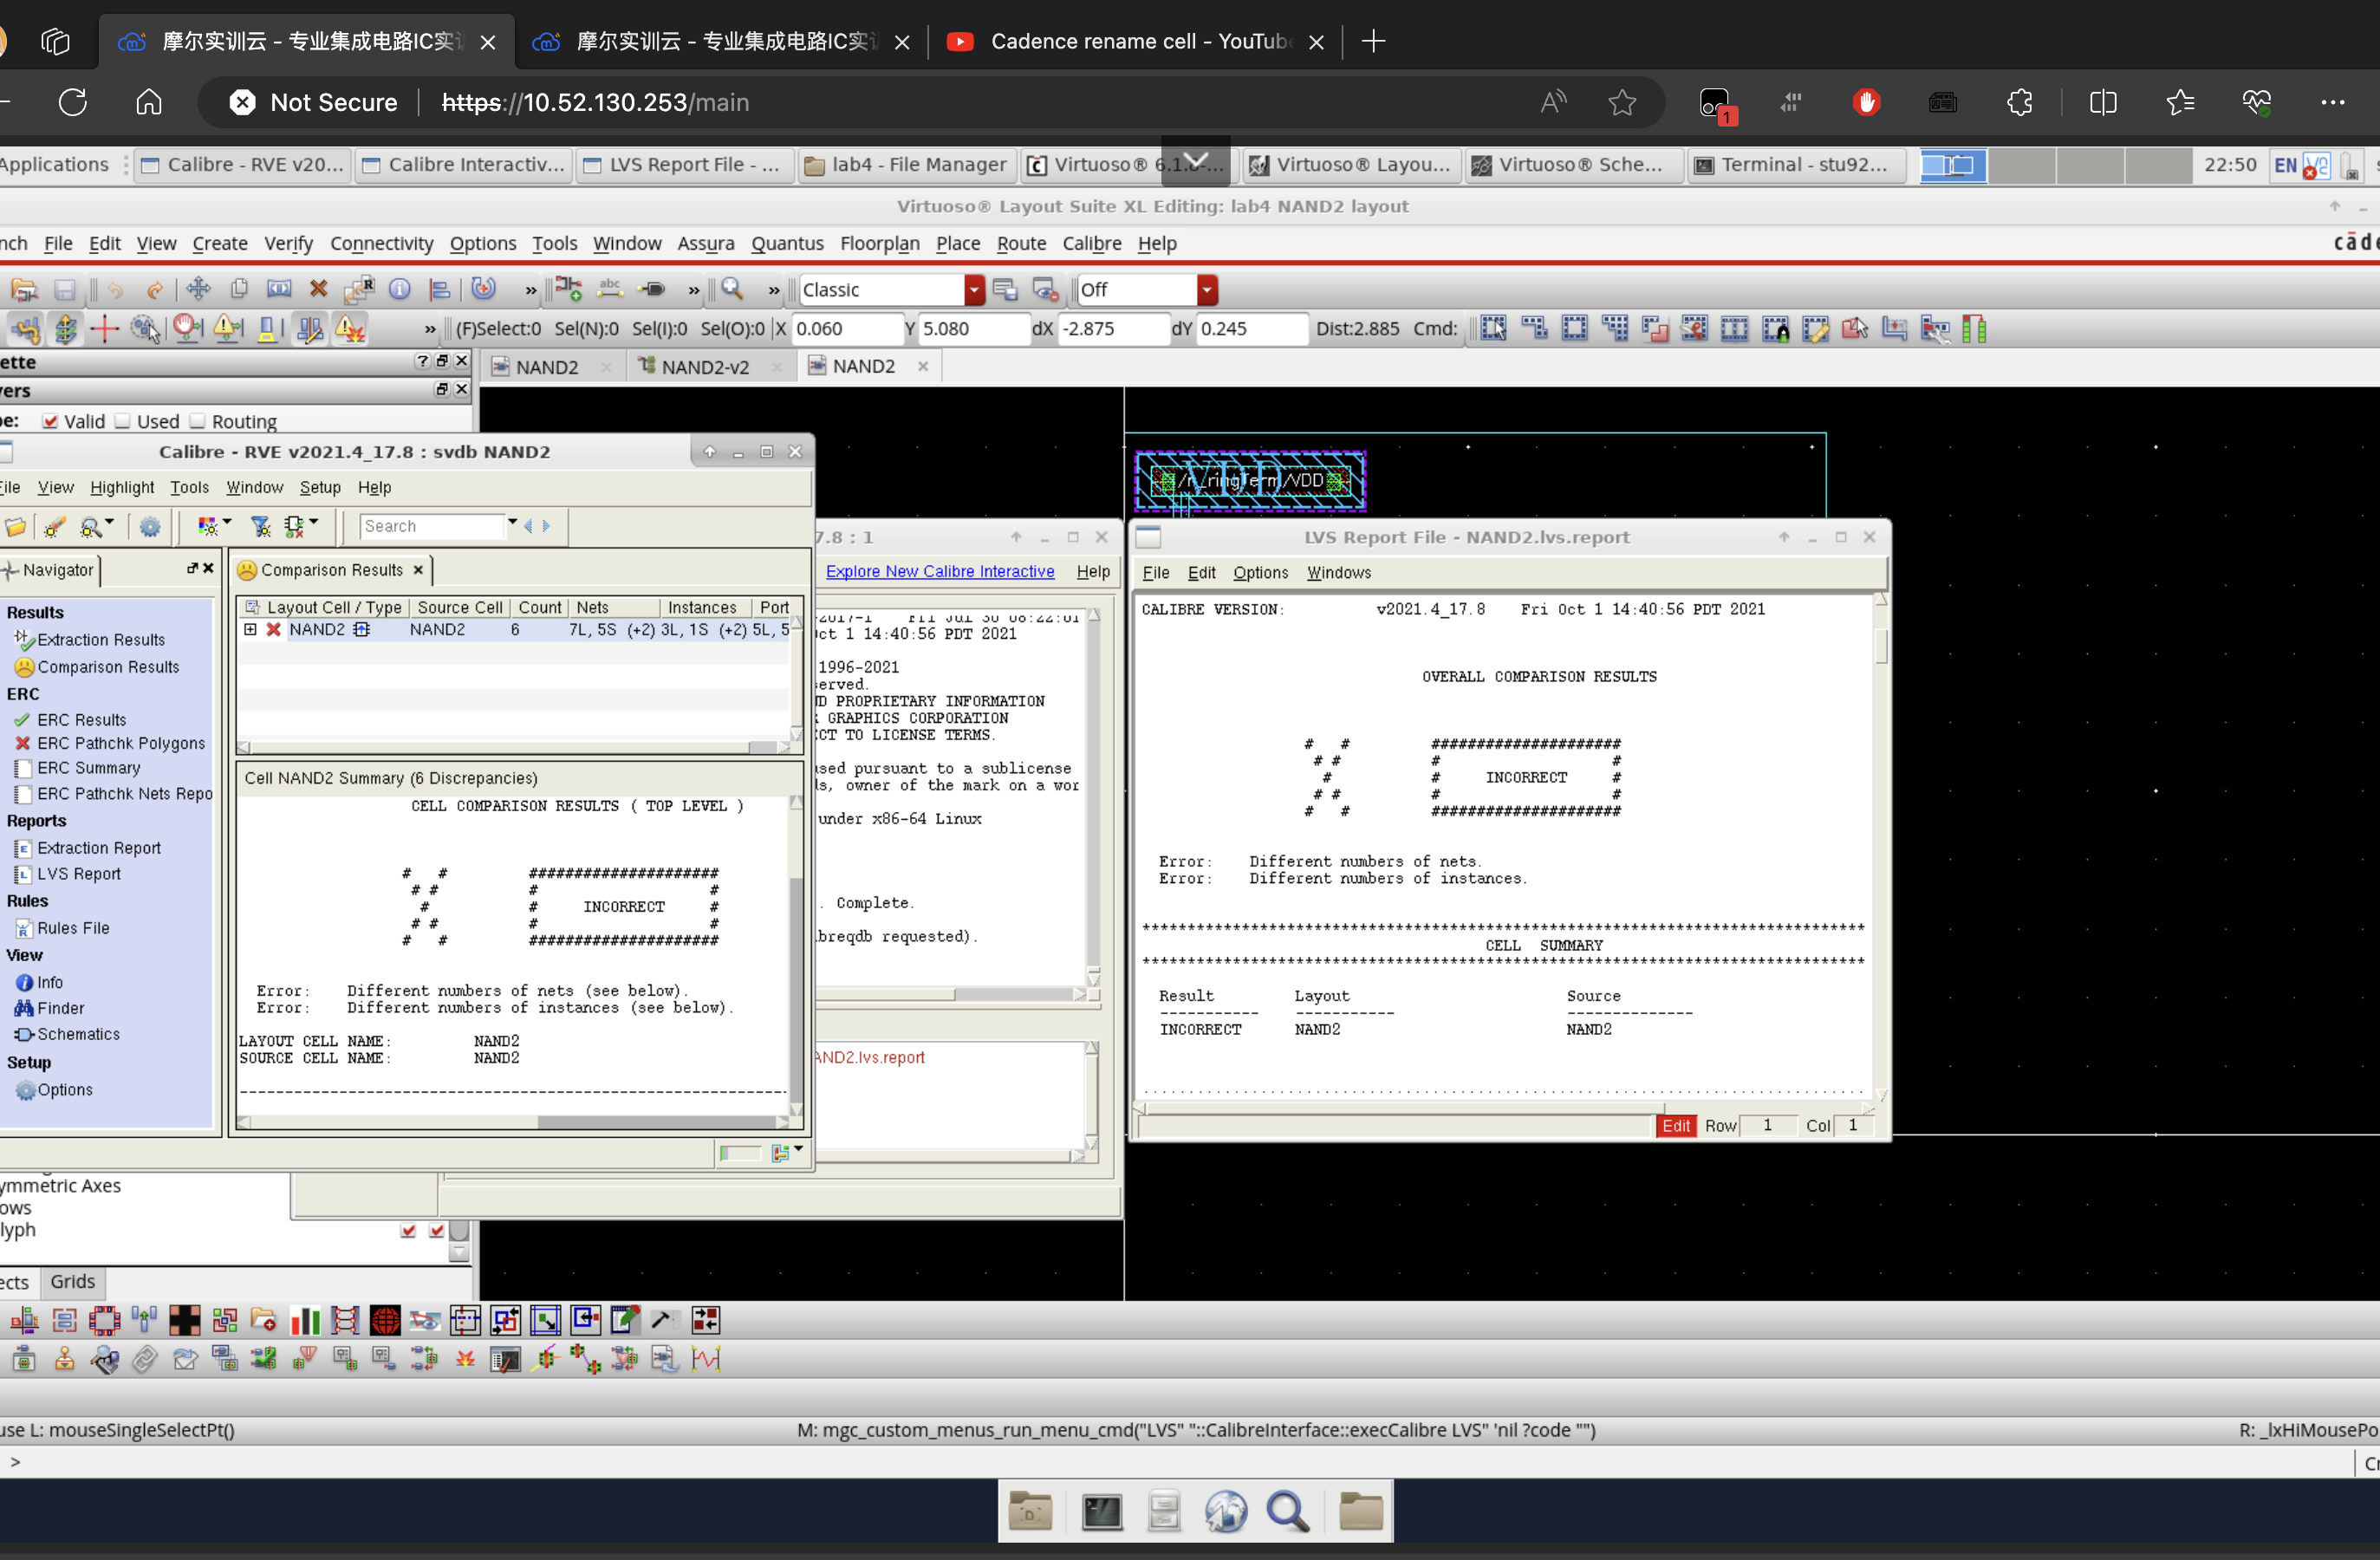
\includegraphics[width=0.6\linewidth]{5-nand2-lvs/nand2-lvs-1.png}
  \caption{nand lvs incorrect}
\end{figure}

经过修改后,再次点击 \texttt{Calibre -> Run nmLVS},可以看到,现在已经没有错误了,出现了笑脸。

\begin{figure}[H]
  \centering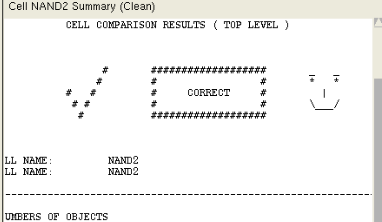
\includegraphics[width=0.6\linewidth]{5-nand2-lvs/nand2-lvs-pass.jpg}
  \caption{nand lvs correct}
\end{figure}

\section{实验总结和感悟}

\subsection{遇到的问题}

LVS NOT COMPARED

Error: Different number of ports.
Error: Power or ground net missing.

\href{https://bbs.eetop.cn/thread-965098-1-1.html}{[求助] lvs结果只显示 Not compared怎么弄?????}

\subsection{实验感想}

通过本次实验,我学会了如何使用 Cadence Virtuoso Layout 进行版图设计,以及如何进行 DRC 和 LVS 检查。在实验中,我遇到了一些问题,比如在 DRC 检查中,我发现 M1 区域的最小面积是 0.2um,而我们的 M1 区域的面积还不到 0.2um,所以我需要调整一下。在 LVS 检查中,我发现了一些错误,经过修改后,最终通过了 LVS 检查。

\subsection{参考资料}

快捷键补充说明

\begin{enumerate}
  \item \href{https://www.cse.psu.edu/~kxc104/class/cse577/11s/hw/hw1/CadenceLayoutShortKey.pdf}{Cadence Virtuoso Layout - A Short Introduction}
  \item \href{https://miscircuitos.com/cadence-keyboard-shortcuts-keybinds-go-faster/}{List of useful Cadence keyboard Shortcuts or Hotkeys for Virtuoso}
\end{enumerate}

如果想要在 Virtuoso Layout 中拖动整个画面,可以按住鼠标中键(或者按住 Shift 键并点击鼠标左键),然后移动鼠标来平移整个视图。这样就可以在画布上自由移动,而不仅仅是移动器件。

\end{document}
